\title{NNPDF}
\author[Christopher Schwan]{}
\institute{Universit\`a di Milano}
\date{PDF4LHC}

\subsection{NLO EW corrections for PDF fits}

\begin{frame}{NLO EW corrections for PDF fits}
\begin{columns}[onlytextwidth]
\begin{column}{0.45\textwidth}

\begin{block}{What do we need?}
\begin{itemize}
\item[\ding{51}] At least QED corrections in DGLAP
\item[\ding{55}] NLO EW (including NLO QCD+EW) corrections for all PDF processes
\end{itemize}
\end{block}

\vspace*{0.7cm}

\begin{block}{Motivation?}
\begin{itemize}
\item In principle: always add EW corrections when we have them, more precision
\item In practice: cuts can be relaxed: DY large-mass region, \ldots
\item Requested at PDF4LHC for a long time
\end{itemize}
\end{block}
\end{column}
\begin{column}{0.45\textwidth}
\begin{block}{Problems to be solved}
\begin{itemize}
\item[\ding{51}] Need corrections in the form of \alert{interpolation grids}: PineAPPL, interfacing with Madgraph5\_aMC@NLO (see \href{https://arxiv.org/abs/2008.12789}{arXiv:2008.12789})
\item[\ding{51}] Careful selection of data: no subtraction of FSR, no photon-initiated subtraction, proper observable definition
\item[\ding{55}] Produce all predictions and implement all (changed) data (WIP)
\item[$\rightarrow$] Run fit
\end{itemize}
\end{block}
\end{column}
\end{columns}
\end{frame}

\begin{frame}{Example: Drell--Yan @ 14 TeV}
\begin{columns}[T,onlytextwidth]
\begin{column}{0.5\textwidth}
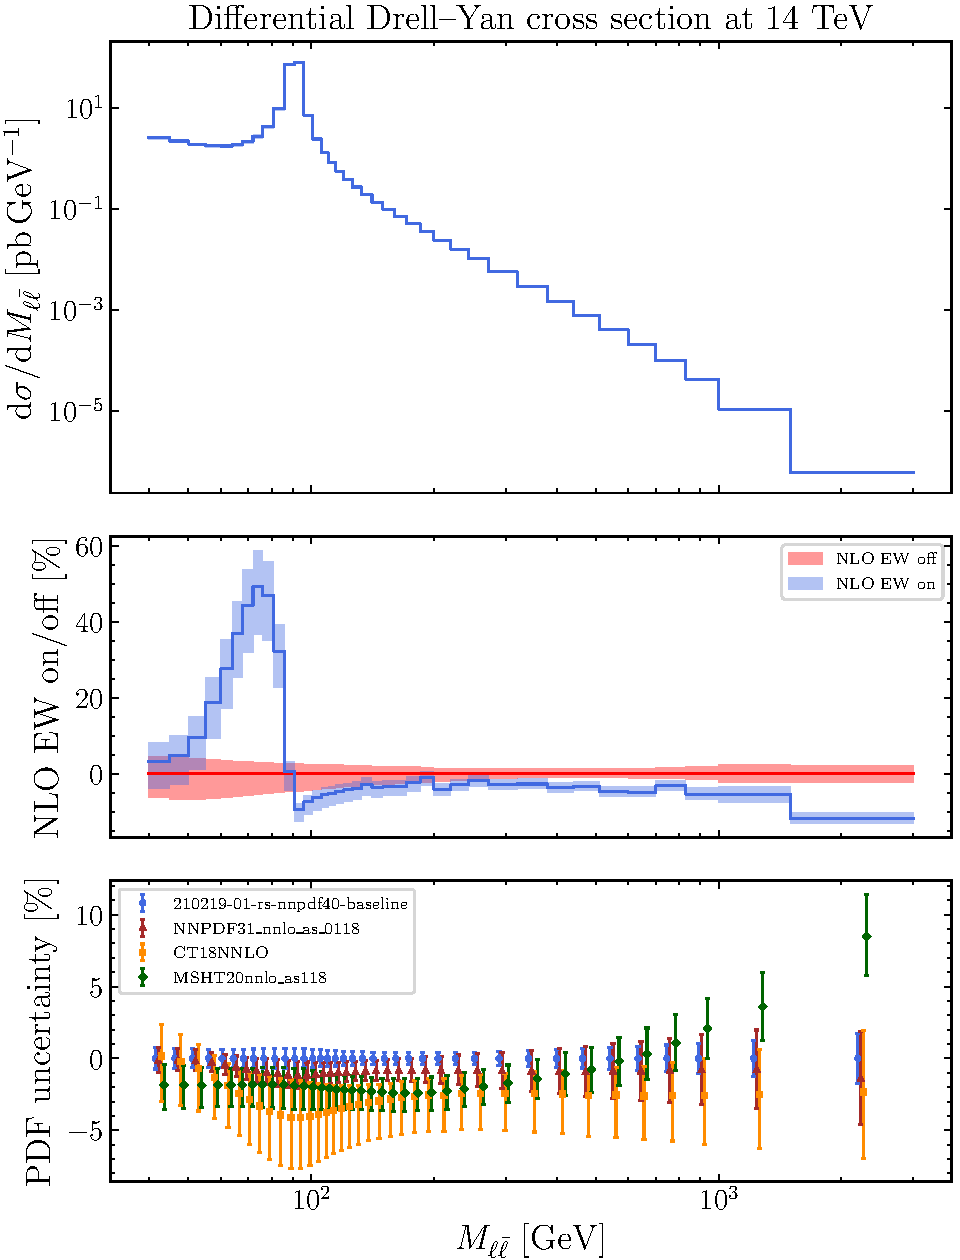
\includegraphics[height=.9\textheight]{ew_corrections/figures/NNPDF40_DY_Z}
\end{column}
\begin{column}{0.5\textwidth}
\begin{itemize}
\vspace*{0.1cm}
\item binning from CMS DY @ \SI{13}{\tera\electronvolt}: \href{https://arxiv.org/abs/1812.10529}{arXiv:1812.10529}
\vspace*{2.3cm}
\item FSR distort the Z peak, weak corrections in the large-mass region
\vspace*{1.3cm}
\item PDF uncertainties for NNPDF4.0, 3.1, CT18NNLO, and MSHT20
\end{itemize}
\end{column}
\end{columns}
\end{frame}
